\chapter{GCSE Revision - Straight Line Equations}

\begin{enumerate}
  \item Finding a gradient
  \begin{enumerate}
    \item What is the gradient of the line that goes through the points $(1,6)$ and $(5,-3)$.\strch
    \item What is the gradient of the line $x + 2y = 1$?\strch
  \end{enumerate}
  \item Finding the equation of the line given two points.
  \begin{enumerate}
    \item Give the full equation of the line which goes through the points $(3,5)$ and $(5,11)$.\strch
    \item Give the full equation of the line which goes through the points $(5,1)$ and $(8,-8)$.\strch
    \item Give the full equation of the line which has the gradient 4 and goes through the point $(0,3)$.\strch
    \item Give the equation of the line which has gradient 4 and goes through the point $(3,7)$.\strch
  \end{enumerate}
  \newpage
  \item Finding the equation of a line parallel or perpendicular to another.
  \begin{enumerate}
    \item Give the equation of the line which is parallel to $y = 4x + 3$ and goes through the point $(4,5)$.\strch
    \item Give the equation of the line which is parallel to $y = \frac{1}{3} x - 2$ and goes through the point $(9,5)$.\strch
    \item Give the equation of a line which is perpendicular to $y = 2x + 1$.\strch
    \item Give the equation of the line which is perpendicular to $y = 5x + 6$ and goes through the point $(-15,2)$.\strch
  \end{enumerate}
  \item Finding where a line intercepts the $x$ or $y$ axis.
  \begin{enumerate}
    \item The y-axis:\strch
    \item The x-axis:\strch
  \end{enumerate}
  \newpage
  \item At what point does $y = 3x - 2$ intercept:
  \begin{enumerate}
    \item The y-axis: \strch
    \item The x-axis: \strch
  \end{enumerate}
  \item A and B are straight lines. Line A has equation $2y = 3x + 8$. Line B goes through the points $(-1, 2)$ and $(2, 8)$. Do lines A and B intersect? You must show all your working.\mrk{3}\strch
  \item \mbox{}
  \begin{figure}[H]
    \centering
    \begin{tikzpicture}[>=latex, scale=0.8]
      \tkzDefPoints{-1/0/X1, 6/0/X2, 0/-2.5/Y1, 0/6/Y2, 0/-1.5/P, 5/2/B}

      \tkzDrawSegment[->](X1,X2)
      \tkzDrawSegment[->](Y1,Y2)

      \tkzInterLL(P,B)(X1,X2)
      \tkzGetPoint{A}

      \tkzDefLine[perpendicular=through A](P,B)
      \tkzGetPoint{d}

      \tkzInterLL(A,d)(Y1,Y2)
      \tkzGetPoint{D}

      \tkzDefLine[perpendicular=through D](D,A)
      \tkzGetPoint{c1}

      \tkzDefLine[perpendicular=through B](A,B)
      \tkzGetPoint{c2}

      \tkzInterLL(B,c2)(D,c1)
      \tkzGetPoint{C}

      \tkzDrawSegments(P,B A,D D,C B,C)
      \tkzMarkRightAngles(D,A,B A,B,C B,C,D C,D,A)

      \tkzLabelPoints[below left](P)
      \tkzLabelPoints[below](A)
      \tkzLabelPoints[right](B)
      \tkzLabelPoints[above](C)
      \tkzLabelPoints[left](D)
    \end{tikzpicture}
  \end{figure}
  $ABCD$ is a square. $P$ and $D$ are points on the $y$-axis. $A$ is a point on the $x$-axis. $PAB$ is a straight line.\\
  The equation of the line that passes through the points $A$ and $D$ is $y = -2x + 6$. Find the length of $PD$.\mrk{4}\strch
  \newpage
  \item \mbox{}
  \begin{figure}[H]
    \centering
    \begin{tikzpicture}[>=latex, scale=0.8]
      \tkzDefPoints{-4/0/X1, 4/0/X2, 0/-4/Y1, 0/4/Y2, -0.6/1/A, 3/3.5/B, 7/3/L}

      \tkzDrawSegment[->](X1,X2)
      \tkzDrawSegment[->](Y1,Y2)

      \tkzDrawPoints[shape=cross out, size=4pt](A,B)

      \tkzLabelPoint[above left](A){A(-1,2)}
      \tkzLabelPoint[above right](B){B(7,5)}

      \tkzLabelPoint[above](L){Diagram \textbf{NOT}}
        \tkzLabelPoint[below](L){accurately drawn}
    \end{tikzpicture}
  \end{figure}
  $A$ is the point $(-1, 2)$. $B$ is the point $(7, 5)$.
  \begin{enumerate}
    \item Find the coordinates of the midpoint of $AB$.\mrk{2}\strch \\\vspace*{0pt}\hfill(\dline,\dline)
    \suspend{enumerate}
      $P$ is the point $(-4, 4)$\\
      $Q$ is the point $(1, -5)$
    \resume{enumerate}
    \item Find the gradient of $PQ$.\mrk{2}\strch \\\vspace*{0pt}\hfill(\dline,\dline)
  \end{enumerate}
  \newpage
  \item \mbox{}
  \begin{figure}[H]
    \centering
    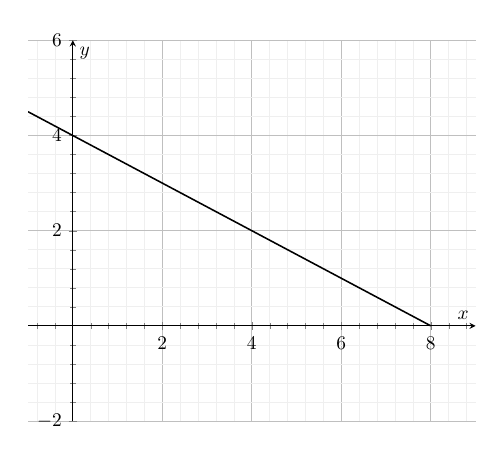
\begin{tikzpicture}[scale=0.7]
      \begin{axis}[
          xmin = -1, xmax = 9,
          ymin = -2, ymax = 6,
          grid = both,
          minor tick num = 4,
          major grid style = {lightgray},
          minor grid style = {lightgray!25},
          axis lines = middle,
          width = 0.8\textwidth,
          height = 0.7\textwidth,
          xlabel = {$x$},
          ylabel = {$y$},
        ]
        % Plot a function
        \addplot[
          domain = -1:8,
          samples = 200,
          smooth,
          thick,
        ] {(8 - x)/2};
        \end{axis}
      \end{tikzpicture}
    \end{figure}
    The graph of the straight line $x + 2y = 8$ is shown on the grid.
    \begin{enumerate}
      \item On the grid, draw the graph of $y = x/2 - 1$.\mrk{3}\strch
      \item Use the graphs to find estimates for the solution of\mrk{1}
      \begin{flalign*}
        &x + 2y = 8\\
        &y = \frac{x}{2} - 1
      \end{flalign*}\strch
    \end{enumerate}\hfill x= \dline, y = \dline
    \newpage
    \item On the grid, draw the graph of $y = 4x - 2$
    \begin{figure}[H]
      \centering
      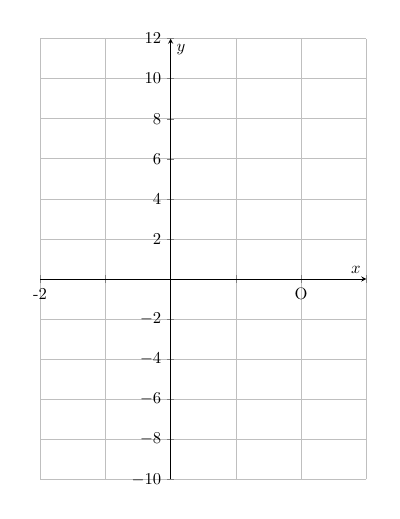
\begin{tikzpicture}[scale=0.6]
        \begin{axis}[
            xmin = -2, xmax = 3,
            ymin = -10, ymax = 12,
            grid = both,
            xticklabels = {{}, {-2}, {}, {-1}, {}, {O}, {},  {1}, {}, {2}, {}, {3}},
            axis lines = middle,
            width = 0.7\textwidth,
            height = 0.9\textwidth,
            xlabel = {$x$},
            ylabel = {$y$},
          ]
          \end{axis}
        \end{tikzpicture}
      \end{figure}
      \begin{enumerate}
        \item Find the gradient of the straight line with equation $2x - 3y = 12$.\mrk{2}\strch\\\vspace*{0pt}\hfill\dline
        \item Prove that the straight line with equation $2y = 10 - 3x$ is perpendicular to the straight line with equation $2x - 3y = 12$.\mrk{2}\strch\\\vspace*{0pt}\hfill\dline
      \end{enumerate}
      \newpage
      \item %
      \begin{enumerate}
        \item Complete the table of values for $3x + 2y = 6$.\mrk{2}
        \begin{table}[H]
          \centering
          \begin{tabularx}{0.75\textwidth} { 
              | >{\centering\arraybackslash}X 
              | >{\centering\arraybackslash}X 
              | >{\centering\arraybackslash}X 
              | >{\centering\arraybackslash}X
              | >{\centering\arraybackslash}X
              | >{\centering\arraybackslash}X
              | >{\centering\arraybackslash}X| }
            \hline
            x	& -2 & -1 &	0 &	1 &	2 &	3 \\
            \hline
            y	& &	4.5 &	3 & & & -1.5 \\
            \hline
          \end{tabularx}
        \end{table}
        \item On the grid, draw the graph of $3x + 2y = 6$.\mrk{2}
        \begin{figure}[H]
          \centering
          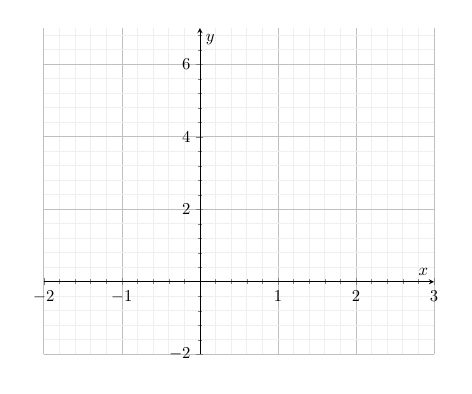
\begin{tikzpicture}[scale=0.6]
            \begin{axis}[
                xmin = -2, xmax = 3,
                ymin = -2, ymax = 7,
                grid = both,
                minor tick num = 4,
                major grid style = {lightgray},
                minor grid style = {lightgray!25},
                axis lines = middle,
                height = 0.7\textwidth,
                xlabel = {$x$},
                ylabel = {$y$},
              ]
              \end{axis}
            \end{tikzpicture}
          \end{figure}
        \item Find the gradient of the graph of $3x + 2y = 6$.\mrk{2}.\strch\\\vspace*{0pt}\hfill\dline
      \end{enumerate}
      \item The diagram shows the graph of $y = x^2 - 5x - 3$
      \begin{figure}[H]
        \centering
        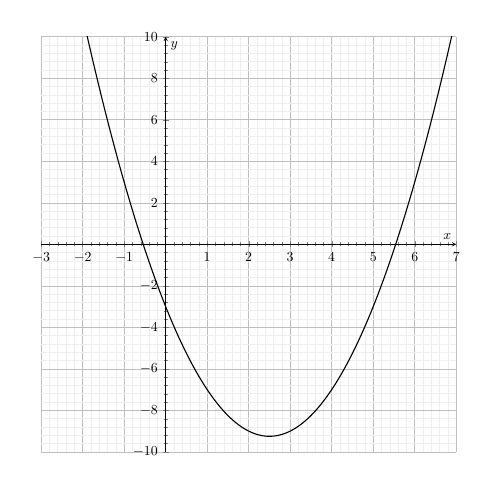
\begin{tikzpicture}[scale = 0.5]
          \begin{axis}[
              xmin = -3, xmax = 7,
              ymin = -10, ymax = 10,
              grid = both,
              minor tick num = 4,
              major grid style = {lightgray},
              minor grid style = {lightgray!25},
              axis lines = middle,
              width = \textwidth,
              height = \textwidth,
              xlabel = {$x$},
              ylabel = {$y$},
            ]
            % Plot a function
            \addplot[
              domain = -2:7,
              samples = 200,
              smooth,
              thick,
            ] {x^2 - 5*x - 3};
            \end{axis}
          \end{tikzpicture}
        \end{figure}
        \newpage
        \begin{enumerate}
          \item Use the graph to find estimates for the solutions of\mrk{3}
          \begin{enumerate}
            \item $x^2 - 5x - 3 = 0$\strch\\\vspace*{0pt}\hfill\dline
            \item $x^2 - 5x - 3 = 6$\strch\\\vspace*{0pt}\hfill\dline
          \end{enumerate}
          \item Use the graph to find estimates for the solutions of the simultaneous equations\mrk{3}
          \begin{flalign*}
            y &= x^2 - 5x - 3\\
            y &= x - 4
          \end{flalign*}\hfill\dline
        \end{enumerate}
        \item %
        \begin{figure}[H]
          \centering
          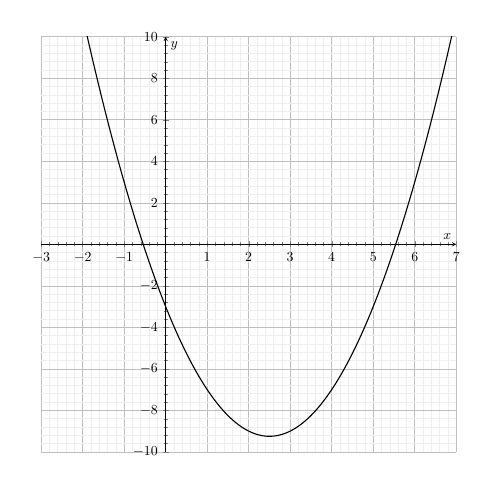
\begin{tikzpicture}[scale = 0.5]
            \begin{axis}[
                xmin = -3, xmax = 7,
                ymin = -10, ymax = 10,
                grid = both,
                minor tick num = 4,
                major grid style = {lightgray},
                minor grid style = {lightgray!25},
                axis lines = middle,
                width = \textwidth,
                height = \textwidth,
                xlabel = {$x$},
                ylabel = {$y$},
              ]
              % Plot a function
              \addplot[
                domain = -2:7,
                samples = 200,
                smooth,
                thick,
              ] {x^2 - 5*x - 3};
              \end{axis}
            \end{tikzpicture}
        \end{figure}
        \newpage
        \begin{enumerate}
          \item Use the graph to find estimates for the solutions of\mrk{3}
          \begin{enumerate}
            \item $x^2 - 5x - 3 = 0$\strch\\\vspace*{0pt}\hfill\dline
            \item $x^2 - 5x - 3 = 6$\strch\\\vspace*{0pt}\hfill\dline
          \end{enumerate}
          \item Use the graph to find estimates for the solutions of the simultaneous equations\mrk{3}
          \begin{flalign*}
            y &= x^2 - 5x - 3\\
            y &= x - 4
          \end{flalign*}\hfill\dline
        \end{enumerate}
        \item \mbox{}
        \begin{figure}[H]
          \centering
          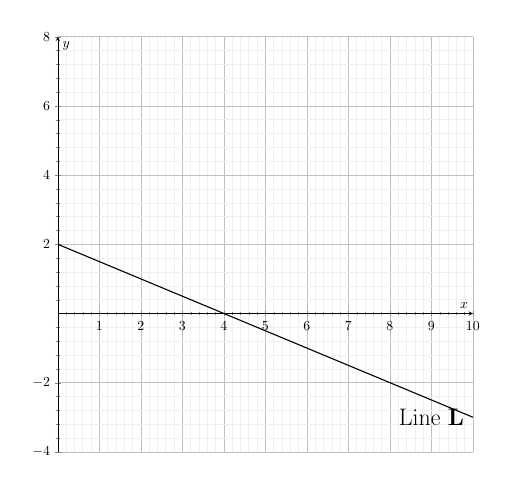
\begin{tikzpicture}[scale = 0.5]
            \begin{axis}[
                xmin = 0, xmax = 10,
                ymin = -4, ymax = 8,
                grid = both,
                minor tick num = 4,
                major grid style = {lightgray},
                minor grid style = {lightgray!25},
                axis lines = middle,
                width = \textwidth,
                height = \textwidth,
                xlabel = {$x$},
                ylabel = {$y$},
              ]
              % Plot a function
              \addplot[
                domain = -0:10,
                samples = 200,
                smooth,
                thick,
              ] {-x/2 + 2};
              \node (A) at (9,-3) {\LARGE Line \textbf{L}};
              \end{axis}
            \end{tikzpicture}
          \end{figure}
          Line \textbf{L} is drawn on the grid.
          \newpage
          \begin{enumerate}
            \item Work out the gradient of Line \textbf{L}.\mrk{2}\strch\\\vspace*{0pt}\hfill\dline
            \suspend{enumerate}
              Another line, Line \textbf{M}, is parallel to Line \textbf{L} and passes through the point $(6, 2)$.
            \resume{enumerate}
            \item Find an equation for Line \textbf{M}.\mrk{2}\strch\\\vspace*{0pt}\hfill\dline
          \end{enumerate}
          \item A straight line passes through $(0, -2)$ and $(3, 10)$. Find the equation of the straight line.
          \begin{figure}[H]
            \centering
            \begin{tikzpicture}[>=latex, scale=0.8]
              \tkzDefPoints{-1/0/X1, 5/0/X2, 0/-2/Y1, 0/6/Y2, 0/-1/A, 2.5/3.5/B, 7.5/5/L}
        
              \tkzDrawSegment[->](X1,X2)
              \tkzDrawSegment[->](Y1,Y2)

              \tkzDrawLines[add=0.2 and 0.4](A,B)
              \tkzDrawPoints[shape=cross out, size=5pt](A,B)
        
              \tkzLabelPoint[right=2pt](B){(3,10)}
              \tkzLabelPoint[left=2pt](A){A(0,-2)}
        
              \tkzLabelPoint[above](L){Diagram \textbf{NOT}}
              \tkzLabelPoint[below](L){accurately drawn}
            \end{tikzpicture}
          \end{figure}\strch
\end{enumerate}

